\documentclass[conference]{IEEEtran}

\usepackage{graphicx}
\usepackage[hidelinks]{hyperref}
\usepackage{float}
\usepackage{easy-todo}

\begin{document}

\title{\todo{AB: To formulate title.}}
\maketitle

\listoftodos

\section{Introduction}
ToDo



\section{Background on STM32}

A typical STM32 system consists of two components:
%
\begin{enumerate}
	\item Hardware - STM32 microcontroller (uniprocessor) and sensors.
	\item Software - sensor logic and scheduler, with Super Loop used as the default baseline.
\end{enumerate}


\subsection{STM32 hardware}

An example of the hardware system is shown in Fig.~\ref{fig:stm32_hw}.
%
\begin{figure}[htbp]
	\centering
	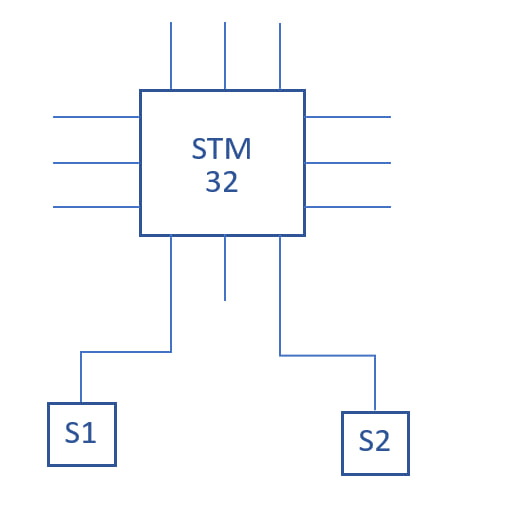
\includegraphics[width=0.8\columnwidth]{STM32_HW.jpg}
	\caption{Hardware components of the STM32 system ($S_1$, $S_2$ - sensors).}
	\label{fig:stm32_hw}
\end{figure}


\subsection{STM32 scheduling}

Super Loop does not account for job deadlines, baseline profiling shows deadline misses and skipped releases under different workload configurations, as shown in Fig.~\ref{fig:superloop_baseline}.

Earliest Deadline First (EDF) as a possible solution accounts for job deadlines, but its performance on STM32 requires experimental evaluation.

The goal is to evaluate schedulability on STM32, identify its main bottlenecks, and improve the scheduling behavior.

This leads to several research ideas:

\begin{enumerate}
	\item Compare EDF and Super Loop scheduling under the same task set
	(\textbf{key metrics:} deadline-miss ratio, skipped-release ratio, response time).
	
	\item Improve EDF behavior under high CPU utilization using feedback control
	(\textbf{key metrics:} deadline-miss ratio, skipped-release ratio, response time, CPU utilization).
	
	\item Minimize unnecessary context switches in EDF
	(\textbf{key metric:} number of preemptions).
\end{enumerate}

\section{Background on Scheduling}

\subsection{Superloop Scheduler: Key Principles}
\begin{figure}[H]
	\centering
	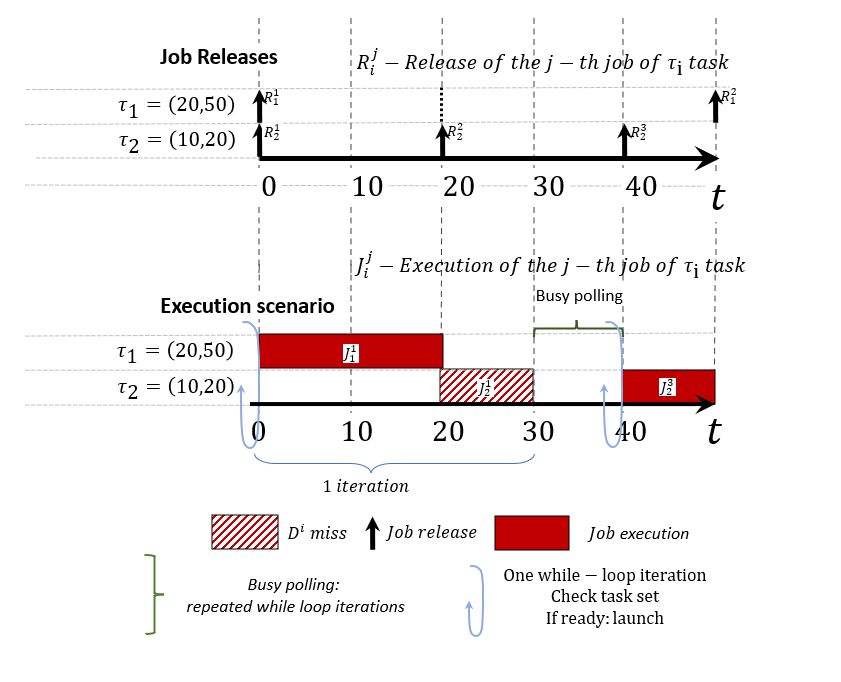
\includegraphics[width=\columnwidth]{SuperLoop ex.png}
	\vspace{0.5em}
	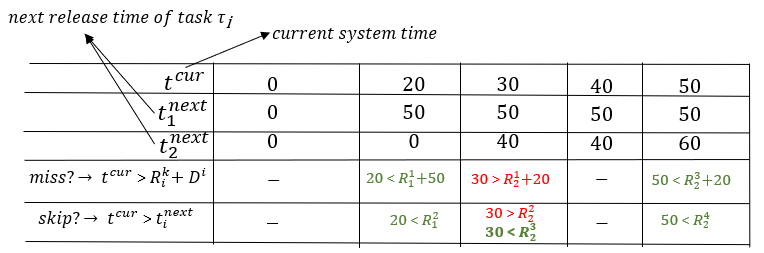
\includegraphics[width=\columnwidth]{SuperLoop table.png}
	\caption{Super Loop execution scenario and corresponding scheduling state.}
	\label{fig:superloop_example}
\end{figure}

\subsection{EDF}
ToDo
\subsection{Brief Comparison}
ToDo (Table)

\section{Schedulers Implementation for STM32}
ToDo (code?)

\section{Performance Evaluation}
\begin{figure}[H]
	\centering
	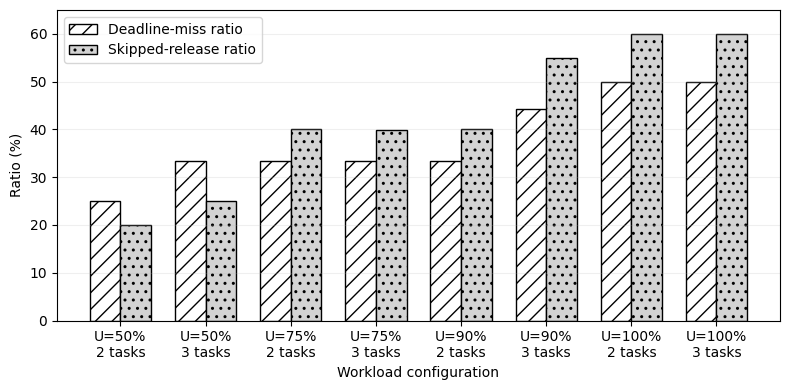
\includegraphics[width=\columnwidth]{SuperLoop.png}
\caption{Super Loop deadline-miss and skipped-release ratios for a specific task under different CPU utilization ($U$) levels and task-set sizes.}
\label{fig:superloop_baseline}
\end{figure}

\end{document}